\documentclass[12pt]{article}
\usepackage[utf8]{inputenc}
\usepackage[fleqn]{amsmath}
\usepackage{amssymb}
\usepackage[fleqn]{mathtools}
\usepackage{amsfonts}
\usepackage{lastpage}
\usepackage{tikz}
\usepackage{pdfpages}
\usepackage{gauss}
\usepackage{fancyvrb}
\usepackage{fancyhdr}
\usepackage{graphicx}
\usepackage{boxproof}
\usepackage{a4wide}
\usepackage{daymonthyear}
\usepackage{textcomp}

\def\meta#1{\mbox{$\langle\hbox{#1}\rangle$}}
\def\macrowitharg#1#2{{\tt\string#1\bra\meta{#2}\ket}}

{\escapechar-1 \xdef\bra{\string\{}\xdef\ket{\string\}}}

\def\intro#1{{#1}{\cal I}}
\def\elim#1{{#1}{\cal E}}

\showboxbreadth 999
\showboxdepth 999
\tracingoutput 1
\definecolor{listinggray}{gray}{0.9}
\usepackage{listings}
\lstset{
	language=,
	literate=
		{æ}{{\ae}}1
		{ø}{{\o}}1
		{å}{{\aa}}1
		{Æ}{{\AE}}1
		{Ø}{{\O}}1
		{Å}{{\AA}}1,
	backgroundcolor=\color{listinggray},
	tabsize=3,
	rulecolor=,
	basicstyle=\scriptsize,
	upquote=true,
	aboveskip={0.2\baselineskip},
	columns=fixed,
	showstringspaces=false,
	extendedchars=true,
	breaklines=true,
	prebreak =\raisebox{0ex}[0ex][0ex]{\ensuremath{\hookleftarrow}},
	frame=single,
	showtabs=false,
	showspaces=false,
	showstringspaces=false,
	identifierstyle=\ttfamily,
	keywordstyle=\color[rgb]{0,0,1},
	commentstyle=\color[rgb]{0.133,0.545,0.133},
	stringstyle=\color[rgb]{0.627,0.126,0.941},
 	literate={\$}{{\textcolor{blue}{\$}}}1,
}
\let\imp\to
\def\elim#1{{{#1}{\cal E}}}
\def\intro#1{{{#1}{\cal I}}}
\def\lt{<}
\def\eqdef{=}
\def\eps{\mathrel{\epsilon}}
\def\biimplies{\leftrightarrow}
\def\flt#1{\mathrel{{#1}^\flat}}
\def\setof#1{{\left\{{#1}\right\}}}
\let\implies\to
\def\KK{{\mathsf K}}
\let\squashmuskip\relax
\pagestyle{fancy}
\fancyfoot[C]{\footnotesize Page \thepage\ of 10}
\DeclareGraphicsExtensions{.pdf,.png,.jpg}
\author{Nikolaj Dybdahl Rathcke}
\chead{Nikolaj Dybdahl Rathcke (rfq695)}

\begin{document}
\section*{Logic in Computer Science - Assignment 5}
\subsection*{3.4.7}
\subsubsection*{a}
We want to prove the set identity $[[\top]]=S$.\\
\\
This holds by definition as seen in clause 1.

\subsubsection*{b}
We want to prove the set identity $[[\bot]]=\emptyset$.\\
\\
Again using clause 1, it holds as we see $s\not\models\bot$ meaning there is no $s\in S$ for which it holds. That means it must be the empty set so we can write $[[\bot]]=\emptyset$.

\subsubsection*{c}
We want to prove the set identity $[[\neg\phi]]=S-[[\phi]]$.\\
\\
From clause 3, we see that $s\models\neg\phi$ if and only if $s\not\models\phi$ in our model. This means, given an entire universe $S$, it must be in all the sets where $[[\phi]]$ is not true. So we can write $[[\neg\phi]]=S-[[\phi]]$.

\subsubsection*{d}
We want to prove the set identity $[[\phi_1\land\phi_2]]=[[\phi_1]]\cap [[\phi_2]]$.\\
\\
From clause 4, $s\models \phi_1\land\phi_2$ when $s\models\phi_1$ and $s\models\phi_2$ in our model. This means that $s$ must be in the set where $[[\phi_1]]$ holds and in the set where $[[\phi_2]]$ is true. Thus it must be in intersection of $\phi_1$ and $\phi_2$, so we write $[[\phi_1\land\phi_2]]=[[\phi_1]]\cap[[\phi_2]]$.

\subsubsection*{e}
We want to prove the set identity $[[\phi_1\lor\phi_2]]=[[\phi_1]]\cup [[\phi_2]]$.\\
\\
From clause 5, $s\models \phi_1\lor\phi_2$ when $s\models\phi_1$ or $s\models\phi_2$ in our model. This means that $s$ must be in the set where $[[\phi_1]]$ holds or the set where $[[\phi_2]]$ is true. Thus it must be in union of $\phi_1$ and $\phi_2$, so we write $[[\phi_1\lor\phi_2]]=[[\phi_1]]\cup[[\phi_2]]$.
\newpage
\subsubsection*{f}
We want to prove the set identity $[[\phi_1\to\phi_2]]=(S-[[\phi_1]])\cup [[\phi_2]]$.\\
\\
From clause 6, $s\models \phi_1\to\phi_2$ when $s\not\models\phi_1$ or $s\models\phi_2$ in our model. From (c) we know we can rewrite the first condition as $S-[[\phi_1]]$. Now, we also know from (e) that the \texttt{or} operator between two formula can be written as the union set of the two. Thus, we can write $[[\phi_1\to\phi_2]]=(S-[[\phi_1]])\cup [[\phi_2]]$.

\subsection*{3.4.10}
\subsubsection*{a}
We want to determine if the CTL formulas $EF\phi$ and $EG\phi$ are equivalent.\\
\\
These are not equivalent. Consider the following model and let $\phi=s$
\begin{center}
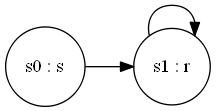
\includegraphics[scale=0.75]{graph1}
\end{center}
Then $EF\phi$ is true in the path $\pi=s_0\to (s_1)^*$ but $EG\phi$ can never be true.

\subsubsection*{b}
We want to determine if the CTL formulas $EF\phi\lor EF\psi$ and $EF(\phi\lor\psi)$ are equivalent.\\
\\
Yes, they are equivalent. \\
To show this, consider that $s\models EF\phi \lor EF\psi$. We can now assume that $s\models EF\phi$ (or $s\models EF\psi$). Now, if we know that is a path including $\phi$ or $\psi$, this means that path also includes $\phi\lor\psi$ which means $s\models EF(\phi\lor\psi)$.\\
If we consider that $s\models EF(\phi\lor\psi)$, then we know that there is a path including $\phi\lor\psi$. This means there must exists a path with $\phi$ or there is a path with $\psi$, which is the same as $s\models EF\phi \lor EF\psi$

\newpage
\subsubsection*{c}
We want to determine if the CTL formulas $AF\phi\lor AF\psi$ and $AF(\phi\lor\psi)$ are equivalent.\\
\\
These are not equivalent. Consider the following model and let $\phi=s$ and $\psi=r$.
\begin{center}
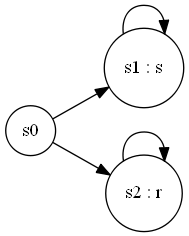
\includegraphics[scale=0.75]{graph2}
\end{center}
In this model, $AF\phi\lor AF\psi$ can not be true as there is a path that does not include $s$ in the first condition and the same for the other condition where there is a path where $r$ is not included.\\
However, $AF(\phi\lor\psi)$ is always true as there exists no path that does not include either $s$ or $r$.

\subsection*{NuSMV Exercise}
\subsubsection*{1}
The NuSMV code implementing this can be seen in appendix A1 or in file \texttt{NuSMVExercise.smv}

\subsubsection*{2}
The specifications can be seen in the \texttt{main} module. The specification for \textit{safety} is as follows
\begin{center}
AG !((p0.label = l5) \& (p1.label = l5))
\end{center}
Where l5 is the line for the critical section. This captues the property as it should always hold (for all paths and globally) that \textit{\textbf{not}} both processes can be in the critical section (l5) at the same time.\\
The specification for \textit{liveness} is as follows
\begin{center}
AG ((p0.label in {l1,l2,l3,l4}) $\to$ AF (p0.label = l5))
\end{center}
This captures the liveness property as it says that it must always hold that if $p0$ is in the lines before the critical section then it follows it always will be in the critical section at some point.\\
The process $p1$ is not included as it is symmetric to $p0$.

\subsubsection*{3}
The output is seen in appendix A2. The explanations are not told as in the output, but merely summarized.\\
For the safety specification:\\
\\
$p0$ goes into the critical section since turn is $0$.\\
$p1$ goes into the loop where it checks the flag of $p0$.\\
$p0$ sets its flag to false.\\
$p1$ goes out of the loop but does not yet set turn to $1$.\\
$p0$ sets its flag to true and and since turn is $0$ it goes into the critical section again.\\
$p1$ sets turn to $1$ and can now go into the critical section as well.\\
\\
For the liveness specification:\\
\\
$p0$ goes into the critical section as turn is $0$.\\
$p0$ goes out of the critical section as sets its flag to false.\\
$p1$ now enters the 'turn-loop' and 'flag-loop' and leaves the flag-loop as it was false.\\
$p0$ sets its flag to true.\\
$p1$ sets turn to $1$ and enters the critical section.\\
$p0$ enters the flag-loop asince turn is $1$.\\
$p1$ sets its flag to false, then sets it to true and enters the critical section as turn again.\\
$p0$ is still in the flag-loop as $p1$ has it flag to true.\\
\\
The last two lines are looped and whenever $p0$ has to do something, then $p1$'s flag is true so there is nothing to do.

\newpage
\section*{A1}
\begin{verbatim}
MODULE main
VAR
  turn  : {0,1};
  flag  : array 0..1 of boolean;
  p0    : process prc(turn, flag, 0);
  p1    : process prc(turn, flag, 1);
-- safety
SPEC AG !((p0.label = l5) & (p1.label = l5));
-- liveness
SPEC AG ((p0.label in {l1,l2,l3,l4}) -> AF (p0.label = l5));

MODULE prc(turn, flag, id)
VAR
  label : {l1,l2,l3,l4,l5,l6,l7};
ASSIGN
  init(label)   := l1;
  init(flag[id]):= TRUE;
  next(label)   :=
    case
      (label = l1)                          : l2;
      (label = l2) & (turn = 0) & (id = 0)  : l5;
      (label = l2) & (turn = 1) & (id = 1)  : l5;
      (label = l2) & (turn = 1) & (id = 0)  : l3;
      (label = l2) & (turn = 0) & (id = 1)  : l3;
      (label = l3) & (flag[1])  & (id = 0)  : l3;
      (label = l3) & !(flag[1]) & (id = 0)  : l4;
      (label = l3) & (flag[0])  & (id = 1)  : l3;
      (label = l3) & !(flag[0]) & (id = 1)  : l4;
      (label = l4)                          : l2;
      (label = l5)                          : l6;
      (label = l6)                          : l7;
      (label = l7)                          : l1;
    esac;
  next(turn)    :=
    case
      (label = l4)                : 1 - turn;
      TRUE                        : turn;
    esac;
  next(flag[id]):=
    case
      (label = l1)                : TRUE;
      (label = l6)                : FALSE; 
      TRUE                        : flag[id];
    esac;
FAIRNESS running
\end{verbatim}

\newpage
\section*{A2}
\begin{verbatim}
-- specification AG !(p0.label = l5 & p1.label = l5)  is false
-- as demonstrated by the following execution sequence
Trace Description: CTL Counterexample
Trace Type: Counterexample
-> State: 1.1 <-
  turn = 0
  flag[0] = TRUE
  flag[1] = TRUE
  p0.label = l1
  p1.label = l1
-> Input: 1.2 <-
  _process_selector_ = p0
  running = FALSE
  p1.running = FALSE
  p0.running = TRUE
-> State: 1.2 <-
  p0.label = l2
-> Input: 1.3 <-
-> State: 1.3 <-
  p0.label = l5
-> Input: 1.4 <-
-> State: 1.4 <-
  p0.label = l6
-> Input: 1.5 <-
  _process_selector_ = p1
  p1.running = TRUE
  p0.running = FALSE
-> State: 1.5 <-
  p1.label = l2
-> Input: 1.6 <-
-> State: 1.6 <-
  p1.label = l3
-> Input: 1.7 <-
  _process_selector_ = p0
  p1.running = FALSE
  p0.running = TRUE
-> State: 1.7 <-
  flag[0] = FALSE
  p0.label = l7
-> Input: 1.8 <-
  _process_selector_ = p1
  p1.running = TRUE
  p0.running = FALSE
-> State: 1.8 <-
  p1.label = l4
-> Input: 1.9 <-
  _process_selector_ = p0
  p1.running = FALSE
  p0.running = TRUE
-> State: 1.9 <-
  p0.label = l1
-> Input: 1.10 <-
-> State: 1.10 <-
  flag[0] = TRUE
  p0.label = l2
-> Input: 1.11 <-
-> State: 1.11 <-
  p0.label = l5
-> Input: 1.12 <-
  _process_selector_ = p1
  p1.running = TRUE
  p0.running = FALSE
-> State: 1.12 <-
  turn = 1
  p1.label = l2
-> Input: 1.13 <-
-> State: 1.13 <-
  p1.label = l5
-- specification AG (p0.label in ((l1 union l2) union l3) union l4 -> AF p0.labe
l = l5)  is false
-- as demonstrated by the following execution sequence
Trace Description: CTL Counterexample
Trace Type: Counterexample
-> State: 2.1 <-
  turn = 0
  flag[0] = TRUE
  flag[1] = TRUE
  p0.label = l1
  p1.label = l1
-> Input: 2.2 <-
  _process_selector_ = p0
  running = FALSE
  p1.running = FALSE
  p0.running = TRUE
-> State: 2.2 <-
  p0.label = l2
-> Input: 2.3 <-
-> State: 2.3 <-
  p0.label = l5
-> Input: 2.4 <-
-> State: 2.4 <-
  p0.label = l6
-> Input: 2.5 <-
-> State: 2.5 <-
  flag[0] = FALSE
  p0.label = l7
-> Input: 2.6 <-
-> State: 2.6 <-
  p0.label = l1
-> Input: 2.7 <-
  _process_selector_ = p1
  p1.running = TRUE
  p0.running = FALSE
-> State: 2.7 <-
  p1.label = l2
-> Input: 2.8 <-
-> State: 2.8 <-
  p1.label = l3
-> Input: 2.9 <-
-> State: 2.9 <-
  p1.label = l4
-> Input: 2.10 <-
  _process_selector_ = p0
  p1.running = FALSE
  p0.running = TRUE
-> State: 2.10 <-
  flag[0] = TRUE
  p0.label = l2
-> Input: 2.11 <-
  _process_selector_ = p1
  p1.running = TRUE
  p0.running = FALSE
-> State: 2.11 <-
  turn = 1
  p1.label = l2
-> Input: 2.12 <-
-> State: 2.12 <-
  p1.label = l5
-> Input: 2.13 <-
  _process_selector_ = p0
  p1.running = FALSE
  p0.running = TRUE
-- Loop starts here
-> State: 2.13 <-
  p0.label = l3
-> Input: 2.14 <-
  _process_selector_ = main
  running = TRUE
  p0.running = FALSE
-- Loop starts here
-> State: 2.14 <-
-> Input: 2.15 <-
  _process_selector_ = p1
  running = FALSE
  p1.running = TRUE
-> State: 2.15 <-
  p1.label = l6
-> Input: 2.16 <-
  _process_selector_ = p0
  p1.running = FALSE
  p0.running = TRUE
-> State: 2.16 <-
-> Input: 2.17 <-
  _process_selector_ = p1
  p1.running = TRUE
  p0.running = FALSE
-> State: 2.17 <-
  flag[1] = FALSE
  p1.label = l7
-> Input: 2.18 <-
-> State: 2.18 <-
  p1.label = l1
-> Input: 2.19 <-
-> State: 2.19 <-
  flag[1] = TRUE
  p1.label = l2
-> Input: 2.20 <-
-> State: 2.20 <-
  p1.label = l5
\end{verbatim}

\end{document}